\Week{4}{Proving the Existence : The Probabilistic Method}

The probabilistic method is a simple and powerful technique to show that some combinatorial object with certain properties exists. The idea is quite simple, design a random experiment to obtain the combinatorial object and then show that the probability that the properties does not get satisfied with probability strictly less than 1. Hence, by probability arguments, there must exist the combinatorial object having the properties in the underlying sample space.

\section{Hypergraph 2-coloring}

Now we show the first application of the probablistic method through the example of hypergraph 2-coloring. 
A hypergraph is a pair of two sets $(V,E)$ referred to as vertices and edges (or hyperedges).The edges are subsets of the vertices. If all the sets in $E$ have size $k$, then we call it the $k$-uniform hypergraph. Notice that a graph is a $2$-uniform hypergraph. A proper (vertex) coloring is an assignments of colors to the vertices of a hypergraph so that no edge is monochromatic. Note that this naturally generalizes graph (vertex) coloring where it is insisted that adjacent vertices (that is, the elements of the edges) get different colors.

We show the following theorem using probabilistic method.

\begin{theorem}[\bf Erd\"os~(1963)]
If $H(V,E)$ is a $k$-uniform hypergraph with less than $2^{k-1}$ hyperedges then there exists a proper 2-coloring of $H$.
\end{theorem}
\begin{proof}
Let $H(V,E)$ be a hypergraph such that $|E| < 2^{k-1}$.
The experiment we set up is to color each vertex in the graph with one of the two colors (say red and blue) uniformly at random (that is, with probability $\half$ the vertex will be colored red and with probability $\half$ it will be colored blue). Let $A_e$ be the event that all the $k$ vertices in the hyperedge $e \in E$ gets the same color. We calculate $Pr[A_e]$ first. Since the monochromatic color for $A_e$ can be chosen in two ways: 
$$Pr[A_e] = \frac{2}{2^k} = \frac{1}{2^{k-1}}$$

The coloring is not proper if the event $A_e$ happens for at least one of the hyperedge $e$. Hence, 
$$Pr[\textrm{ coloring is not proper }] \le Pr\left[\bigcup_{e \in E} A_e\right] \le \sum_{e \in E}Pr[A_e] \le \frac{|E|}{2^{k-1}} < 1$$

That is, if we choose a random 2-coloring, we will get a proper-coloring with probability greater than zero. This, in particular implies that there exists a proper $2$-coloring of the hypergraph.
\end{proof}

We remark that by simply restricting $|E| < 2^{k-2}$ we could have proved that if we choose a random 2-coloring, we will get a proper-coloring with probability greater than $\half$. However, this implies that there is even a randomized algorithm to construct the coloring, in this case. Indeed, if we can efficiently derandomize the algorithm, it makes the proof constructive.

The following exercise tells us that the above scheme can also be applied for higher number of colors too.

\begin{exercise}
Suppose $k > 2$ and let $H$ be a $k$-uniform hypergraph with $4^{k-1}$ edges. Show that there is a 4-colouring of $V(H)$ such that no edge is monochromatic.
\end{exercise}

\begin{curiousity}[\textbf{Property-B Conjecture}]
A hypergraph H has \textbf{Property B} (or 2-colorable) if there is a red-blue vertex-coloring with no monochromatic edge. A hypergraph with property B is also called bipartite, by analogy to the bipartite graphs. Erdos (1963) asked: What is the minimum number of edges $m_2(k)$ of a $k$-uniform
hypergraph not having property $B$? Indeed, the above discussion implies that $m_2(k) \ge 2^{k-1}$. Erdos proved an upper bound of $m_2(k) \le O(k^22^k)$. The best known bounds are :
$$\Omega\left(\sqrt{\frac{k}{\ln k}}2^k\right) \le m_2(k) \le O\left(k^22^k\right)$$
The upper bound is due to Erdos (1964) and the lower bound went through a series of improvements to reach the above bound Radhakrishnan and Srinivasan (2000).
$$
\left\{
\begin{array}{c}
m_2(k) \ge \left(\half\right) 2^k \\
\textrm{\cite{Erd63} }
\end{array}
\right\}
\rightarrow
\left\{
\begin{array}{c}
m_2(k) \ge \left(\frac{k}{k+4}\right)2^k \\
\textrm{\cite{Sch64} }
\end{array}
\right\}
\rightarrow
\left\{
\begin{array}{c}
m_2(k) \ge \left(\sqrt[3]{k}\right)2^k \\
\textrm{\cite{Bec78} }
\end{array}
\right\}
\rightarrow
\vspace{-3mm}
\left\{
\begin{array}{l}
m_2(k) \ge \left(\sqrt{\frac{k}{\ln k}}\right)2^k \\[-2mm]
\textrm{[{\color{blue}RS, 2000)}]\nocite{RS00}}
\end{array}
\right\}
$$
It is believed that $k2^k$ is the right asymptotic bound for $m_2(k)$. In fact, this is a conjecture due to Erdos and Lovasz: $m_2(k) \in \Theta(k2^k)$.
\end{curiousity}

\section{Diagonal Ramsey Number Bound}

We now show the original application of the probabilistic method, when it was introduced by Erd\"os. This is to prove a lower bound for certain ramsey numbers. We now quickly introduce Ramsey numbers in this lecture.

The standard starting point is the following brain teaser : any party with at least $6$ people will contain a group of three mutual friends or a group of three mutual non-friends. Indeed, the immediate combinatorial argument goes like this : call the people $1, 2, 3, 4, 5, 6$. Either $1$ has three friends or three non-friends. Without loss of generality, suppose that $2,3,4$ are all friends with $1$. Then if any pair of them are friends with each other, that pair plus $1$ forms a group of three mutual friends. If no two of them are friends, then they are a group of three mutual non-friends. 

Note that the above can also be done graph theoretically where we consider a 6 vertex graph with drawing an edge between two vertices $i,j \in \{1,2,\ldots 6\}$ if and only if they are friends with each other. Now the above argument can be tranlated to graph : \textit{any graph on $6$ vertices will contain either a clique on 3 vertices or an independent set on 3 vertices}.\\[-2mm]

\hspace{-6mm}\begin{minipage}{0.75\textwidth}
An alternate way to represent the above problem is by $2$-coloring the edges of the complete graph $K_6$, by red if the two vertices are friends with each other and with blue otherwise. Now the above statement becomes : {\em in any 2-coloring of $K_n$, there is a monochromatic triangle} - which indeed, is more concise statement.

Is there a peculiarity with $6$ and can the same be argued for $5$? It turns out that we cannot and there is the following counter example (which we represent by the $2$-coloring of $K_5$).
Thus $6$ is the minimum number such that for any $2$-coloring of the edges of $K_6$ there will exist a monochromatic triangle.
\end{minipage}
\begin{minipage}{0.15\textwidth}
\vspace{-3mm}
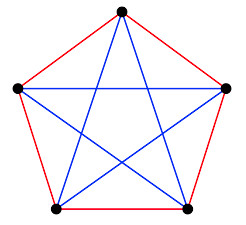
\includegraphics[scale=0.5]{ramsey.jpg}
\end{minipage}

\noindent The Ramsey theory asks a general extremal combinatorics question of this form : For any $s,t \in \mathbb{N}$, what the minimum number $n$ such that there is a guarantee of the form : any $2$-coloring of the edges of the graph $G$ has either a red $K_s$ or a blue $K_t$ in it. This number exists (as proved by Frank Ramsey) and is called the Ramsey Number $R(s,t)$.
In this language, the above argument says $R(3,3) = 6$.
In fact, the existance argument for Ramsey number actually gives the followng upper bound.
\begin{proposition}
$R(s,t) \le R(s,t-1)+R(s-1,t)$.
\end{proposition}

Computing other Ramsey numbers has attracted a lot of attention from combinatorialists. However, we know very little still. $R(s,2)=s$, $43 \le R(5,5) \le 49$ etc. The numbers where $s=t$ are the diagonal entries of the Ramsey matrix (which is natural to imagine given the above). By applyng the above theorem, we have that: $$R(s,s) \le 2^{2s}\sqrt{s}$$

In the rest of this section, we will concetrate on  lower bounds for the diagonal Ramsey numbers. Notice that to show lower bound $R(s,s) \ge n$, we need to show that there is a $2$-coloring of $K_n$ where there is no monochromatic $K_s$. A constructive lower bound of this kind was discovered by Nagy which shows :
$$R(s,s) \ge {s \choose 3}$$

We now apply probabilistic method in order to obtain a stronger lower bound. Erdos, in 1947, introduced
probabilistic methods in his paper {\em Some Remarks on the Theory of Graphs} for proving this lower bound.

\begin{theorem}
The diagonal Ramsey number $R(s,s)$ is at least $\lfloor 2^{\frac{s}{2}}\rfloor$.
Equivalently, when $n=2^{\frac{s}{2}}$, there exists a $2$-coloring of $K_n$ where there is no monochromatic $K_s$.
\end{theorem}
\begin{proof}
As usual, we need to show the existance of a 2-coloring to edges. We set up the following experiment. Color each edge uniformly at random with red or blue. The total number of possible colorings is $2^{n \choose 2}$. The probability of any particular color configuraton is exactly $\frac{1}{2^{n \choose 2}}$.

We need to prove an upper bound of the bad events. Let $S \subseteq n$ of size $s$. Our coloring is bad if $S$ is colored monochromatic under the above coloring.
$$Pr[\textrm{$S$ is monochromatic}] \le \frac{2 \times 2^{{n \choose 2}-{s \choose 2}}}{2^{n \choose 2}} \le 2^{1-{s \choose 2}}$$
$$Pr[\textrm{$\exists S : S$ is monochromatic}] \le
\sum_{S \subseteq [n]:|S|=s} Pr[\textrm{$S$ is monochromatic}] \le {n \choose s}2^{1-{s \choose 2}}$$

If we show that ${n \choose s}2^{1-{s \choose 2}}$ is less than $1$ for $n=2^{s/2}$, then we are done by probablistic argument.

$$
{n \choose s}2^{1-{s \choose 2}} 
\le \frac{n^s}{s!}2^{1-(s/2)+(s^2/s)} 
\le \frac{n^s}{2^{s^2/2}}\frac{2^{1+s/2}}{s!}<1
$$
Hence the proof.
\end{proof}

\begin{exercise-prob}[See Problem Set 2~(Problem~\ref{tournament})]
\begin{show-ps2}{tournament}
A tournament is a directed graph $G(V,E)$ on $n$ vertices where for every pair $(i,j)$, there is either an edge from $i$ to $j$ or from $j$ to $i$, but not both (it represents real tournaments, where we interpret $(i,j)$ directed edge as player $i$ beats player $j$. There is no draw and all pairs of players play a game with each other). 

A tournament T is said to have \textbf{$k$-championship property} if for any set of $k$ vertices in the tournament, there is some vertex in $V$ that has a directed edge to each of those $k$ vertices.

Can $k$-Championship property occur in small tournament graphs? For example, for $k=1$, a tournament will need at least $3$ vertices to have the $k$-Championship property. If $k=2$, a tournament will need at least 5 vertices to have $k$-Championship property.

Show that there are tournments of size $O(k^22^k)$ having $k$-Championship property. [Hint : Consider a random tournament. Fix a set $S$ of $k$ vertices and some vertex $v \notin S$. What is the probability that $v$ is the champion in $S$?]
\end{show-ps2}
\end{exercise-prob}

\begin{exercise-prob}[See Problem Set 2~(Problem~\ref{dominating-set}]
\begin{show-ps2}{dominating-set}
Let $G(V,E)$ be a graph. A set of vertices $D \subseteq V$ is called dominating
with respect to $G$ if every vertex in $V \setminus D$ is adjacent to a vertex in D. $\delta(G)$, the minimum degree amongst $G$’s vertices, is strictly positive. Then $G$ contains a dominating set of size less than or equal to:
$$ \frac{n(1+\log(1+\delta))}{1+\delta} $$
[Hint : Choose a subset $X\subseteq V$ at random (with each vertex in with probability $p$). Let $Y \subseteq V\setminus X$ having no neighbor in $X$. Estimate $X \cup Y$.]
\end{show-ps2}
\end{exercise-prob}

\section{Expectation Method}

We now apply the method of expectation with probablistic method. The basic idea is that when we
want to show the existence of an object for which a parameter (say graph with at least certain number of connected components) satisfy some lower/upper bounds. We first define the parameter as the random variable and show that the expected value satisfies the bounds which implies that there exists an object which satisfies the bounds. The following lemma makes this more precise.

\begin{lemma}[{\bf Expectation Method}]
\label{lem:expectation-method}
For any random variable $X$, 
$$\E[X] \ge t \implies Pr[X \ge t] > 0$$
\end{lemma}

\begin{proof}
Assume for the sake of contradiction that $\Pr[X \ge t] = 0$. 
$$\E[X] = \sum_{w \in \Omega} X(w)P(w)$$
If $\Pr[X \ge t]$ was zero, then by definition, $$\sum_{\substack{w \in \Omega \\ X(w) \ge t}} P(w) = 0$$ 
Since $P(w)$ is non-negative, we have that, for every $w \in \Omega$, with $X(w) \ge t$, $P(w) = 0$.
$$\E[X] = \sum_{w \in \Omega} X(w)P(w) = \sum_{\substack{w \in \Omega \\ X(w) < t}} X(w)P(w) < t \left( \sum_{\substack{w \in \Omega}} P(w) \right) = t$$
That will be a contradiction.

\end{proof}
\noindent Question to students : Does the same statement holds when $\ge$ is replaced by any of $\le,<$ or$ >$ ?

\subsection{Sum-free Sets}

To apply the expectation method, we need to make a suitable choice of the random variable $X$ so that it is not difficult to compute its expected value. We demonstrate thetechnique by using the example of sum-free sets. We start witht he definitions.

A subset $A$ of positive integers is called \textit{sum-free}, if $\not\exists x,y,z \in S$ such that $x+y = z$ (the number may repeat). Given a set of positive integers, say $B = \{b_1,b_2, \ldots b_n\}$ how large a sum-free subset is it guaranteed to contain? 
A simple example to try out is $B = \{1,2,\ldots n\}$. If we choose all odd numbers in the set, or even the elements more than $\frac{n}{2}$, they all are sumfree subsets of size at least $\frac{n}{2}$.
Erd\"os answered this question using a cute mathematical statement.

\begin{theorem}
For any set $B = \{b_1,b_2, \ldots b_n\}$ of positive integers, there must exist a sumfree subset $A \subseteq B$ such that $|A| > \frac{n}{3}$.
\end{theorem}
\begin{proof}
We will follow the above outlined strategy to define an appropriate random variable but in an indirect way. We choose a prime $p > 2b_n$ where $b_n$ is the largest number in $B$ and that $p=3k+2$. Now all addition operation between the elements in $B$ are faithfully  captured in the the set $\Z_p$ where addition is done modulo $p$. That is there is a natural mapping from $B$ to $\Z_p$ which preserves the sum operations. The mapping can be thought of as the identity function since $p \ge 2b_n$. Indeed, $\phi(b_i+b_j) = \phi_(b_i)+\phi(b_j)$ from the definitions itself.

\hspace{-5mm}\begin{minipage}{0.65\linewidth}
{\bf Sum-free sets in $\Z_p$:} Instead of showing a sum-free subset of $B$, we show a sum-free subset $C$ of $\Z_p$ first. We explicitly define $C$ first. Consider the middle third elements of $\Z_p$. That is, $C = \{k+1,k+2, \ldots 2k+1\}$. And $|C| > \frac{p-1}{3}$. We claim that $C$ is sum-free. To see this : $x,y,z \in C$, $x+y \ge 2k+2$ even for the smallest elements in $C$, and $x+y = 4k+2$ (which is at most $k$ modulo $3k+2$) even for the largest elements in $C$. Hence none of these sums will land back in $C$ as a result of the modulo operation. Hence $C$ is sum-free.
\end{minipage}
\begin{minipage}{0.05\linewidth}
~
\end{minipage}
\begin{minipage}{0.25\linewidth}
\vspace{-1cm}
\begin{tikzpicture}[shorten >=0.5pt,node distance=0.2cm,on grid,auto]
\draw (2,0) ellipse (1cm and 2cm) node[midway,yshift=2cm, xshift=2cm]{$B$~~~~~};
\draw (2,0) ellipse (0.7cm and 1.1cm)
node{$A$};;
\draw (5,0) ellipse (1cm and 2.1cm) node[midway,yshift=2cm, xshift=5.1cm]{$\Z_p$~~~~~};
\draw (5,0) ellipse (0.5cm and 1cm)
node{$C$};;
\end{tikzpicture}
\end{minipage}
\vspace{4mm}

\noindent{\bf Pull-back to $B$ - A failed attempt:} Now how do we go back to get a subset of $B$ which is sumfree. A natural idea is to use the "pull back" of the function $\phi$. The pre-image of $C$, namely $\phi^{-1}(C)$ must be sumfree as well. To see this : if there exists $x, y, z \in \phi^{-1}(C)$  such that $x+y = z$, then $\phi(x)+\phi(y) = \phi(z)$. Since $\phi(x),\phi(y),\phi(z) \in C$ by definition, this implies that $C$ is not sumfree and that is a contradiction. But then, why should the size of the pre-image by at least $\frac{n}{3}$? It could even be that none of the elements in $B$ are mapped to $C$, so the pre-image can even be empty !.\\[-3mm]

\noindent{\bf Way forward - random scaling: } Since the above mapping may not be good, we consider variants of $\phi$ which also preserves the addition operation  in $B$. Consider any $\alpha \in \Z_p \setminus \{0\}$, the map $\phi_\alpha : B \to \Z_p$:
$$\phi_\alpha : b_i \mapsto \alpha b_i \mod p$$
Let us quickly check if this is a function which respects the sum operation: if $b_i+b_j = b_k$, $\phi_\alpha(b_i)+\phi_\alpha(b_j)=\alpha b_i \mod p +\alpha b_j \mod p = (\alpha b_i+\alpha b_j) \mod p = \phi_\alpha(b_i+b_j) = \phi_\alpha(b_k)$
As a consequence, the pre-image of $C$ under any $\alpha$, $\phi_\alpha^{-1}(C)$  will be sumfree.

\noindent Now comes the punch line argument. We will argue :
$$\textrm{\em $\exists \alpha \in \Z_p\setminus\{0\}$ such that $\phi_\alpha^{-1}(C)$ is a large subset of $B$.}$$
It is to prove this last statement that we apply the expectation method described above. To begin with, let us write the claim more precisely:
\begin{claim}
$\exists \alpha \in \Z_p\setminus\{0\}$ such that $|\phi_\alpha^{-1}(C)| > n/3$.
\end{claim}

Original statement that we wanted to prove said, $\exists A \subseteq B$, now it says $\exists \alpha \in \Z_p \setminus \{0\}$. Let us set up the experiment.
Choose $\alpha$ uniformly at random from $\Z_p \setminus \{0\}$. Let us defined the random variable $X$ as:
$$X = |\phi_\alpha^{-1}(C)| = |\{ i \in [n] \mid \phi_\alpha(b_i) \in C \}|$$

As per expectation method, we just need to prove that $\E[X] > \frac{n}{3}$. Let us breakdown this random variable into simpler ones in terms of the individual $b_i$s. Let us define the indicator random variable corresponding to the event $\phi_\alpha (b_i) \in C$.

$$X_i^{\alpha} = \left\{
\begin{array}{ll}
1 & \textrm{ if $\phi_\alpha (b_i) \in C$} \\
0 & \textrm{ otherwise}
\end{array}
\right.
$$
Note that, $X = \sum_{i=1}^n X_i$. Hence, by linearity of expectation, $\E[X] = \sum_{i=1}^n \E[X_i^{\alpha}]$. Thus, we need to lower bound $\E[X_i^{\alpha}]$. Since it is an indicator random variable, $\E[X_i^{\alpha}] = \Pr_\alpha\left[\phi_\alpha (b_i) \in C\right]$ which we will compute now.

For a $b_i$ and a a target element on RHS (consider a non-zero element on RHS $y \in \Z_p \setminus \{0\}$) how many $\alpha$ can map $b_i$ to $y$? This is exactly one element $\alpha = b_iy^{-1} \mod p$. Thus, if we choose an $\alpha$ uniformly at random, probability that it maps $b_i$ to $y$ is $\frac{1}{p-1}$. If, in addition, this $y$ has to be in the set $C$, then there are exactly $|C|$ choices of $\alpha$ which sends $b_i$ to $C$. That is:
$$\E[X_i^{\alpha}] = \Pr_\alpha\left[\phi_\alpha (b_i) \in C\right] = \frac{|C|}{p-1} > \frac{1}{3}$$

Thus, as planned, we have shown that $\E[X] = \sum_{i=1}^n \E[X_i^{\alpha}]$ is greater than $\frac{n}{3}$. Hence as per Lemma~\ref{lem:expectation-method} (expectation method), $\Pr_{\alpha}[X \ge \frac{n}{3}] = \Pr_{\alpha}\left[|\phi_\alpha^{-1}(C)| > \frac{n}{3}\right] > 0$. Hence, by probabilistic method, we have that there exists an $\alpha$ such that $|\phi_\alpha^{-1}(C)| > \frac{n}{3}$. Hence there exists an $A$ (namely $\phi_\alpha^{-1}(C)$) which is a subset of $B$ and is sum-free. This completes the argument.
\end{proof}

\subsection{Crossing Number Lower Bound}

Now we discuss a totally different application of expectation which is not necessarily an incarnation of probabilistic method, but still is a fun example.
We set up the context first.

Planar graphs are graphs which can be embedded on the plan without any crossing of the edges. Indeed, there are non-planar graphs. How do we measure non-planarity? There are many ways - one of them is the crossing number of the graph. The crossing number $cr(G)$ of a graph $G$ is the least number of crossings in any embedding of the graph on the plane. Indeed, if the graph $G$ is planar, then $cr(G)=0$. As an exercise, check out the crossing number of the non-planar graphs $K_{3,3}$ and $K_5$. Have fun !.

What can be the bounds on crossing number in terms of the edges and vertices of the graph? Clearly, if the graph is highly dense, then we do expect the crossing number to be high. Hence one should expect a lower bound in terms of the number of edges.

We quickly review the Euler's formula for planar graphs which can also be used to bound the crossing number.

\begin{proposition}[{\bf Euler's Formula for Planar Graphs}]
Any planar graph $G$, with $n$ vertices, $m$ edges and $f$ faces, and $c$ components, must satisfy:
\begin{equation}
n-m+f = c+1
\label{eqn:Euler-formula}
\end{equation}
\end{proposition}
\begin{proof}
The proof is an induction on $m$. If there are no edges ($m=0$), then $f=1$, $c=n$. The formula gets satisfied. Let $m > 0$, and assume that the statement is true for graphs with less than $m$ edges. Consider an edge $e=(u,v)$. Remove this edge from $G$ to obtain a new graph $G'$. Let $c' \ge c$ be the number of components in $G'$. We have two cases:
\begin{description}
\item{\bf Case 1: $c'>c$ : }
The number of components can increase at most bt $1$. $c'=c+1$. By removing the edge, the number of faces does not change since the removed edge would have been the boundary for the outer face of the embedding. Hence $m' = m-1$, $f' = f$. Hence the equation \ref{eqn:Euler-formula} will still be satisfied.
\item{\bf Case 2: $c'=c$ : }
By removing the edge, we would have decreased the number of faces by $1$. Hence $m' = m-1$, $f' = f-1$. Hence the equation \ref{eqn:Euler-formula} will still be satisfied.
\end{description}
\end{proof}

\begin{corollary}
Any connected planar graph $G$ on $n\ge 4$ vertices cannot have more than $3n-6$ edges.
\end{corollary}
\begin{proof}
Let the number of edges in the boundary of the $i^{th}$ face be $m_i$. Observe that each edge can be the boundary of at most two faces. This gives:
$\sum_{i=1}^f m_i \le 2m$. Since $m_i \ge 3$ (even for outer face, since $G$ is connected), this gives $f \le \frac{2m}{3}$. Applying this relation to Euler's formula gives, $m = n+f-2 \le n+\frac{2m}{3}-2$. This gives that $m \le 3n-6$.
\end{proof}
The next corollary is about a lower bound on the crossing number.
\begin{corollary}
\label{cor:euler-crlb}
For any graph with $n$ vertices and $m$ edges, we have that $$cr(G) \ge m-3n+6$$
\end{corollary}
\begin{proof}
The idea is quite simple. Take the best embedding of the graph which achieves the crossing number. For each crossing put in a vertex at the geometric point of the crossing edges. What we get is a planar embedding of a new planar graph $G'$. Indeed the number of vertices have increased by $cr(G)$. The number edges have increased by $2cr(G)$. $n' = n+cr(G)$ and $m' = m+2cr(G)$. Applying the above corollary to the graph $G'$:
$$m+2cr(G) \le 3(n+cr(G)-6$$
This gives that, $cr(G) \ge m-3n+6$, thus completing the proof.
\end{proof}

Thus we have one lower bound for crossing number. We will use our expectation method to derive a much stronger lower bound.

\begin{theorem}[\cite{Bec78}]
Let $G$ be a simple graph with $m > 4n$. Then,
$$cr(G) \ge \frac{1}{64}\frac{m^3}{n^2}$$
\end{theorem}
\begin{proof}
Again, our aim is to define an appropriate experiment and a random variable whose expectation will be lower bounded. Let $G$ be the graph, and let $\tilde{G}$ be the embedding of $G$ on the plane which achieves the crossing number $cr(G)$. That is, the emebedding witnesses $cr(G)$ crossings.

We design the following experiment. Choose a subset of vertices $V$ by choosing each vertex of $G$ independently with probability $p = \frac{4n}{m}$. Let $H$ be the induced subgraph on these vertices and let $\tilde{H}$ be the embedding of $H$ derived from $\tilde{G}$. Notice that $H$ may have a better embedding which achieves a lower crossing number than what $\tilde{H}$ witnesses.

The crossing number of $H$, $cr(H)$ is a random variable. In addition, the number of vertices, number of edges, and the number of crossings of $\tilde{H}$ are all random variable. Let $X,Y,Z$ be these random variables respectively. 

Since $\tilde{H}$ is only one of the possible embeddings of $H$, $Z \ge cr(H)$. Since the number of vertices is independent of the embedding, by applying Corollary~\ref{cor:euler-crlb}, we have that $cr(H) \ge Y-3X$ (we are ignoring the additive constant 6 but the lower bound is still valid), Thus we have that :
$$Z \ge Y-3X \textrm{ which implies that } \E[Z] \ge \E[Y]-3\E[X]$$
Now we need to compute each of them. Since we are choosing each vertex to be in $H$ indendently with probability $p$, $\E[X] = pn$. Since for an edge from $G$ to be chosen, both of its end points must be chosen, $\E[Y] = p^2m$. For a crossing in $\tilde{G}$ to appear in $\tilde{H}$, all the 4 vertices involved in the crossing must be chosen. Hence $\E[Z] = p^4cr(G)$. Plugging this in yields that:
$$p^4cr(G) \ge p^2m - 3pn \implies cr(G) \ge \frac{pm-3n}{p^3} = \frac{n}{(4n/m)^3} = \frac{1}{64}\frac{m^3}{n^2}$$ the required lower bound.
\end{proof}

\begin{exercise-prob}[See Problem Set 2(Problem~\ref{bipartite})]
\begin{show-ps2}{bipartite}
Use expectation method to show that every graph having a matching of size $m$ has a bipartite subgraph with at least $\half(|E(G)|+m)$ edges. (Hint: how can we choose a random bipartition such that the edges of the matching have their endvertices in opposite parts?)
\end{show-ps2}
\end{exercise-prob}

\begin{exercise-prob}[See Problem Set 2(Problem~\ref{designs})]
\begin{show-ps2}{designs}
Let $t,\ell, d \in \mathbb{N}$ and $t \le \ell \le d$. 
A family of sets $S_1, S_2, \ldots S_m \subseteq [d]$ is said to be a $(d,\ell, t)$-design if: 
\begin{itemize}
\itemsep 0pt
\item $\forall i \in [m]$, $|S_i| = \ell$.
\item For all $i,j \in [m], i \ne j$, $|S_i \cap S_j| < t$.
\end{itemize}
That is, the family is $\ell$-uniform (each set of size $\ell$) subsets of $[d]$ with intersection sizes at most $t$. We will have an application soon in the course for such sets. Given $\ell$, we would want maximize the number of sets that can be "packed" in - that is maximise $m$, while keeping $t$ and $d$ to be small. But do such sets exist for all parameters? A typical question that we face in this course, and we use our tools:
\begin{enumerate}[(a)]
\item Prove that if, $m {\ell \choose t}^2 < {d \choose t}$, then there exists an $(d,\ell,t)$-design $S_1, S_2, \ldots S_m \subseteq [d]$. \\
Hint : If the sets are chosen at random, then prove that for every $S_1, S_2, \ldots S_{i-1}$:
$$\E_{S_i}\left[\# j < i : |S_i \cap S_j| \ge t \right] < 1$$
\item Use this to conclude that for every constant $c > 0$, $\ell, m \in \mathbb{N}$, there exists and $(d,\ell,t)$-design, $S_1, S_2, \ldots S_m \subseteq [d]$ with $d = O\left( \frac{\ell^2}{t} \right)$ and $t = c\log m$. In particular, setting $m = 2^\ell$, we can fit exponentially many sets of size $\ell$ in a universe of size $d = O(\ell)$
while keeping the intersections as logarithmically small.
\item Use method of conditional expectations to derandomize the above to show how to construct designs as in Parts 1 and 2 deterministically in time $\poly(m,d)$.
\end{enumerate}
\end{show-ps2}
\end{exercise-prob}


\section{Refined Probablistic Method : Lova\'sz Local Lemma}

In many situations where we apply the probabilistic method, one is trying to show that it is possible to avoid {\em bad events} 
$\calE_1, \calE_2, \ldots \calE_n$ with positive probability. That is, we show that, $\Pr[\bigcap_{i} \overline{\calE_i}] > 0$ where $\overline{\calE_i}$ denotes the complementary event to $\calE$.

One way to show $\Pr[\bigcap_{i} \overline{\calE_i}] > 0$ is to use $\Pr[\bigcap_{i}\overline{\calE_i}] = 1-\Pr[\bigcup_{i}\calE_i]$.
We now use the fact that $\Pr[\bigcup_i \calE_i] \le \sum_i \Pr[\calE_i]$. We try to show that this last sums up to less than $1$. Indeed the last inequality is weak. That is, $\sum_i \Pr[\calE_i]$ may even be more than $1$, but still $\Pr[\bigcup_i \calE_i] < 1$.

If in addition, we knew that the events $\cal_i$ are independent, then it suffices to have that $\Pr[\calE_i] < 1$ for each $i$. Then, $$\Pr[\bigcap_{i} \overline{\calE_i}] = \prod_i (1-\Pr[\calE_i]) > 0$$
Indeed, it might tougher to design independent events whose simultaneous avoidance is enough to estalish the existance of the object that we are looking for.

Hence, we need a framework, where even if $\calE_i$s are dependent, still one can estimate and argue that $\Pr[\bigcap_{i} \overline{\calE_i}]$ is less than $1$. This is what Lov\'asz Local Lemma helps us do, where the dependence is a little more structured.

\subsection{Dependency Graph}

As mentioned above, Lov\'asz Local Lemma helps us to handle the situations where there is only local dependancy. The structure of the dependency between the events under consideration is represented by the dependency graph.

To define the dependency graph, we need the notion of mutual independence which we defined earlier.

\begin{definition}
Let $\calE_1, \calE_2, \ldots \calE_n$ be events. Let $J \subseteq [n]$. We say that event $\calE_i$ is \textit{mutually independent} of the events $\{\calE_j \mid j \in J$ for all $J_1, J_2 \subseteq J$
such that $J_1 \cap J_2 = 0$
$$\Pr [ \calE_i \cap \left( \cap_{j \in J_1} B_j \right) \cap \left( \cap_{j \in J_2} \overline{B_j} \right) ] = \Pr(\calE_i) \Pr[\left( \cap_{j \in J_1} B_j \right) \cap \left( \cap_{j \in J_2} \overline{B_j} \right) ] $$
\end{definition}

Now we are ready to represent the dependency information in the form of a directed graph. The vertices of the graph are the events $\{1,2, \ldots n\}$. 
\begin{definition}[{\bf Dependency Graph}]
A (directed) graph $G([n],E)$ is a dependency graph on events $\calE_1, \calE_2, \ldots \calE_n$
if each event $\calE_i$ is mutually independent of its non-neighbors $\{\calE_j \mid (i,j) \notin E \}$.
\end{definition}

\begin{remark}
Notice that for the same set of events, there can be several dependency graphs. For example, if a directed graph $G$ is a dependency graph for a set of events. If we add more edges to $G$, it will still be a dependency graph for the same set of events.
\end{remark}

\subsection{The Symmetric LLL and an Application}

A simpler version to study first is the symmetric version. In fact, in this version we do not even use the structure of the graph, but only the degree bounds. We first state the lemma:

\begin{lemma}
Suppose $p \in (0,1)$, $d \ge 1$, and $\calE_1, \calE_2, \ldots \calE_n$
are events such that $\Pr[\calE_i] \le p$ for all $i$. If each $E_i$ is mutually independent of all but $d$ other events\footnote{This implies that there is a regular dependency graph} and $ep(d+1) \le 1$, then:
$\Pr[\bigcap_{i} \overline{\calE_i}] > 0$
\end{lemma}

We will prove the symmetric version in the next section. But before that we apply it. We apply to it the hypergraph 2-coloring problem that we talked as the first example for probablistic method. 

\vspace{-4mm}
\paragraph{Application to Hypergraph 2-coloring:}
We demonstrate that, we can still prove a $k$-uniform hypergraph is $2$-colorable even if it has more than $2^{k-1}$ edges (a condition which we required to establish $2$-colorability using Probablistic method) if there is some structural property for the edges : \textit{every edge intersects at most $d$ other edges}.

To apply the lemma, let us think of events $\calE_i$ in the same way : whether the $i^{th}$ edge $e_i$ is monochromatically colored or not. As we did in that example, we have that 
$$\Pr[\calE_i] = \frac{2}{2^k} = \frac{1}{2^{k-1}} = p$$

We now claim that the dependency condition is satisfied. Clearly for a vertex which corresponds to the event of monochromatic coloring of the set $\calE_i$, the other events which does not even have a common vertex with $\calE_j$ are clearly independent of the event $\calE_i$. Hence each event is dependent on at most $d$ other events and hence the degree is upper bounded by $d$. We can always add additional edges to make the graph $d$-regular. The last condition that needs to be checked is whether the individual event probability is low enough.
$$ep(d+1) = e(d+1)\frac{1}{2^{k-1}} \le 1 \textrm{as required by the lemma, if we ensure that $d < \frac{2^{k-1}}{e}-1$}$$

This gives the following theorem.

\begin{theorem}
For any $k$-uniform hypergraph with the guarantee that every hyperedge intersects with at most $2^{k-3}$ other hyperedges, then the hypergraph is $2$-colorable.
\end{theorem}
\begin{exercise-prob}[See Problem Set 1(Problem~\ref{lll})]
\begin{show-ps1}{lll}
For a set of Boolean variables $x_1, x_2, \ldots x_n$, a $k$-CNF formula $\phi$ has the form $\phi = C_1 \land \ldots \land C_m$. Each clause $C_j$ is an or of some set of $k$ literals, where each literal is either $x_i$ or $x_i$ for some $i \in [n]$. Clauses $C_j$ and $C_k$ are said to intersect if $\exists x_i$ such that both clauses contain either $x_i$ or $\lnot x_i$. A satisfying assignment is a setting of the $x_i$s that makes $\phi$ evaluate to true. Deciding the existence of a satisfying assignment for a Boolean CNF formula is another well-studied (and $\NP$-complete) problem. This problem asks you to show that a satisfying assignment exists in certain cases. If each clause intersects at most $\frac{2^k}{e}-1$ other clauses, then show that $\phi$ is satisfiable. (Hint: Use LLL).
\end{show-ps1}
\end{exercise-prob}

\subsection{The Asymmetric LLL and an Application}

We state and prove the general version of LLL and prove it first. We will also show an application of the lemma.

\begin{theorem}[{\bf Lov\'asz Local Lemma}]
Suppose $\calE_1, \calE_2, \ldots \calE_n$ are $n$ events with $G$ as a depedency graph.
If there exists $x_1, x_2, \ldots x_n \in [0,1)$ such that for every $i \in [n]$:
\begin{equation}
\Pr[\calE_i] \le x_i \prod_{(i,j)\in E}(1-x_j)
\label{eqn:LLL-premise}
\end{equation}
then, $$\Pr\left[\bigcap_{i=1}^n \overline{\calE_i}\right] \ge \prod_{i=1}^{n}(1-x_i) > 0$$
\end{theorem}

An important example is when the events are actually independent. In this case the LLL result is tight.
Also, while trying to apply LLL to a situation, having designed the set of events we have the design freedom for the depedency graph and the values $x_1, x_2, \ldots x_n \in(0,1)$. 

\paragraph{Deriving the Symmetric LLL:}
The dependency graph is $d$-regular. Choose $x_i = 1/(d+1)$. With this, we want to show that the premise of the LLL (Equation~\ref{eqn:LLL-premise}) is satisfied.
Indeed, the RHS is $(d+1)(1-\frac{1}{d+1})^{d} \ge \frac{1}{(d+1)e} \ge p \ge \Pr[\calE_i]$. Hence the symmetric version follows.

\paragraph{Proof of the Asymmetric LLL:}
Staring at $\Pr\left[\bigcap_{i=1}^n \overline{\calE_i}\right]$ indicates that may be one can grow the probability bound starting from thinner intersections. To do this, we will define, for $S \subseteq [n]$,
$$\P(S) = \Pr\left[\bigcap_{i\in S} \overline{\calE_i}\right]$$
Clearly, on one side, we have that $P(\phi)=1$, and on the other side we want to derive $P([n])$. This calls for a proof by induction on the size of $|S|$. Thus we strengthen the statement to the following lemma which we prove by induction. Note that the following lemma implies the LLL.

\begin{lemma}
Let $S \subseteq [n]$. For any $i \in S$: 
$$\P(S) \ge \P(S\setminus\{i\})(1-x_i)$$
\end{lemma}
\begin{proof}
Base case is trivial (figure this out !). We will assume the statement holds true whenever $|S|\le k$ and then we will prove it for $|S|=k+1$. Let $S$ be a subset of $[n]$ of size $k+1$ and fix $i \in S$. We need to appeal to indepedence of the events in $S$ for which we need the neighborhood.
$$\Gamma(i) = \{j \mid (i,j) \in E \} \textrm{ ~~and~~ } \Gamma^+(i) = \{i\} \cup \Gamma(i)$$

We need to estimate a lower bound for $P(S)$. We use the fact that for any event $A$, $\Pr[A] = \Pr[A \cap B]+\Pr[A \cap \overline{B}]$. Use $A = 
\bigcap_{i\in S\setminus\{i\}} \overline{\calE_i}$ and $B=\calE_i$. This gives:
\begin{eqnarray*}
\P(S) = \Pr\left[\bigcap_{i\in S} \overline{\calE_i}\right] & = & \Pr[A] - \Pr[A \cap B] \\
& = & \Pr\left[\bigcap_{i\in S\setminus\{i\}} \overline{\calE_i} \right] - 
\Pr\left[\calE_i \cap \bigcap_{i\in S\setminus\{i\}}\overline{\calE_i} \right] \\
& \ge & 
\Pr\left[\bigcap_{i\in S\setminus\{i\}} \overline{\calE_i} \right] - 
\Pr\left[\calE_i \cap \bigcap_{i\in S\setminus\{\Gamma^+(i)\}}\overline{\calE_i} \right] \\
& = & 
\Pr\left[\bigcap_{i\in S\setminus\{i\}} \overline{\calE_i} \right] - 
\Pr[\calE_i]\Pr\left[\bigcap_{i\in S\setminus\{\Gamma^+(i)\}}\overline{\calE_i} \right] \\[3mm]
& = & 
\P[S\setminus\{i\}]-\Pr[\calE_i]\P[S\setminus\Gamma^+(i)]
\end{eqnarray*}

Dividing by $\P[S\setminus\{i\}]$,
\[ \frac{\P(S)}{\P[S\setminus\{i\}]} = 1-\Pr[\calE_i]\frac{\P[S\setminus\Gamma^+(i)]}{\P[S\setminus\{i\}]} \]

Since we are only involving elements from $S$, we can trstrict our attention to the neighbors who are in $S$. Let $\Gamma(i) \cap S = \{b_1,b_2, \ldots b_d\}$. Now the second term can be simplified.
$$\frac{\P[S\setminus\Gamma^+(i)]}{\P[S\setminus\{i\}]} = \frac{\P[S\setminus\{i,b_1\}]}{\P[S\setminus\{i\}]}\times
\frac{\P[S\setminus\{i,b_1,b_2\}]}{\P[S\setminus\{i,b_1\}]}\times
\frac{\P[S\setminus\{i,b_1,b_2,b_3\}]}{\P[S\setminus\{i,b_1,b_2\}]}\times
\cdots
\frac{\P[S\setminus\{i,b_1,b_2,b_3,\ldots,b_n\}]}{\P[S\setminus\{i,b_1,b_2,\ldots,b_{n-1}\}]}
$$
Applying induction hypothesis to each of the terms in the RHS,
$$\frac{\P[S\setminus\Gamma^+(i)]}{\P[S\setminus\{i\}]} \le \prod_{t \in \Gamma(i) \cap S} \frac{1}{(1-x_j)} 
$$
Thus, \[ \frac{\P(S)}{\P[S\setminus\{i\}]} \ge 1-x_i \]
and hence the proof.
\end{proof}


\paragraph{Application : Lower bounds for Ramsey Number:}
The application to Ramsey number is for the number $R(3,\ell)$. By the recurrence relation, it can be shown that $R(3,\ell) \le \frac{\ell(\ell+1)}{2}$. We will obtain a lower bound for $R(3,\ell)$. The result is as follows.
\begin{theorem}
For $\ell \ge 3$, there is a constant $c$ such that:
$$R(3,\ell) \ge \frac{c\ell^2}{\log^2 \ell}$$
\end{theorem}
\begin{proof}
Since we are provinga lower bound, we should show that for $n$ taken as the RHS of the theorem, there exists a $2$-coloring that does not have a red triangle and a blue $t$-clique.

Let $n$ be the number of vertices, which we will fix later. Consider a complete graph on $n$ vertices and a random coloring of its edges with the colors red and blue: We color each edge red with probability $p$ and blue with probability $1-p$; independently for all edges.\footnote{Value of $n$ and $p$ will be spelt out later as expressions in terms of $\ell$.}. We will want to prove that the probability that there is no red triangle and no blue $K_\ell$ is greater than $0$.
\paragraph{Designing the Events:} As planned, we will come up with bad events whose absence will imply the structure that we want. Indeed, bad events are : 
\begin{itemize}
\item for $T \subseteq [n]$, $|T|=3$, $A_T$ is the event where vertices in $T$ are colored with red color.
\item for $S \subseteq [n]$, $|S|=\ell$, $B_S$ is the event where vertices in $S$ are colored with blue color.
\end{itemize}
We can also estimate the probabilities of these events. Indeed, $\Pr[A_T] \le p^3$ and $\Pr[B_S] \le (1-p)^{\ell \choose 2}$. Also, $\overline{A_T}$ for all $T \subseteq [n]$ of size $3$ and $\overline{B_S}$ for all $S \subseteq [n]$ of size $\ell$ implies that there is a $2$-coloring which leaves no red triangle and blue $\K_\ell$ as monochromatic. The number of vertices in the event graph is ${n \choose 3}+{n \choose \ell}$. 

\paragraph{Dependency graph:} We now talk about the dependency graph. The above events are vertices. We add an edge between two events if their corresponding index sets intersect in more than one vertex (to get a common edge). That is an $(A_T,A_{T'}) \in E$ if and only if $|T \cap T'| > 1$ - and similarly for $(B_S,B_{S'}) \in E$ and for the cross edges $(A_T,B_S)$. Notice that this satisfies the dependency relation as well. If there is no common edge between the index sets, then the corresponding events are independent too.

We estimate the degree of each vertex in the graph. Consider a vertex of type $A_T$ where $T=\{u,v,w\}$. Each vertex can have the $A$-type neighbors and $B$-type neighbors. We will count the neighbours of $A$-type first. For each edge $e$ in the triangle $T$, there can only be one more $A_{T'}$ such that $T \cap T'$ is exactly those two vertices. Hence the number $A$-type neighbors that $A_{T}$ vertex can have, is at most $3n$.

We will count the $B$-type neighbors rather loosely. It can at most be the number of $B$-type vertices itself, which is ${n \choose \ell}$. Thus,
$$deg(A_T) \le 3n+{n \choose \ell}$$
By similar consideration, for any $S \subseteq [n]$ with $|S|=\ell$.
$$deg(B_S) \le n{\ell \choose 2}+{n \choose \ell}$$

\paragraph{Satisfying the LLL premise:} 
We now need to choose $x_i$'s in LLL. Let us change to a convenient notation. We will call the $x_i$s corresponding to $A$-type vertices of the dependency graph as $x$ (we will choose all of them to be equal) and $B$-type vertices as the $y$s (we will choose all of them to be equal). Thus we have the following task in hand:

\noindent {\bf Task:} We need to design $n$, $p$ and $x,y \in (0,1)$ such that the inequalities (using the fact that $\Pr(A_T)=p^3$ and $\Pr[B_S] = (1-p)^{\ell \choose 2}$:
\begin{eqnarray}
p^3 \le x(1-x)^{3n}(1-y)^{n \choose \ell}\\
\label{eqn:LLL1}
(1-p)^{\ell \choose 2} \le y(1-x)^{n{\ell \choose 2}}(1-y)^{n \choose \ell}
\label{eqn:LLL2}
\end{eqnarray}

Staring at the expression $(1-y)^{n \choose \ell}$ hints that we should choose $y=\frac{1}{{n \choose \ell}}$ so that this expression can be replaced by roughly $\frac{1}{e}$.

Now since $x$ and $y$ are in $(0,1)$, Equation~\ref{eqn:LLL1} gives us two inequalities.

$$p^3 \le x \textrm{~~and~~} p^3 \le (1-x)^{n \choose \ell}$$

Using the fact that $(1-t)$ is roughly $e^{-t}$, the second equation gives, $p \ge xn \ge p^3$. Thus $p \ge \frac{1}{\sqrt[3]{n}}$
And Equation~\ref{eqn:LLL2} gives us two inequalities.

$$(1-p)^{\ell \choose 2} \le (1-x){n{\ell \choose 2}}
\textrm{~~and~~}(1-p)^{\ell \choose 2} \le y = \frac{1}{{n \choose \ell}} = e^{-\ell\log n}
$$
Applying $(1-t)$ is roughly $e^{-t}$ again, $p{\ell \choose 2} \ge \ell \log n$. Using $p \ell^2 \ge p{\ell \choose 2}$ this gives, $\ell \ge \frac{\log n}{p} \ge \sqrt{n} \log n$. Motivated by these considerations, now we directly give the values for the variables involved.
$$n = \frac{\ell^2}{40\log^2 \ell} \textrm{~~and~~} p = \frac{1}{3\sqrt{n}}$$
$$x = \frac{1}{9n^{3/2}}\textrm{~~and~~}
y =  \frac{1}{{n \choose \ell}}$$
The constants are chosen to offset the error terms in the approximations considered. We leave it as an exercise to check that the inequalities are indeed satisfied.

Hence we have argued that for $n=\frac{\ell^2}{40\log^2 \ell} \textrm{~~and~~} p = \frac{1}{3\sqrt{n}}$, we have a choice of the parameters of $x$ and $y$ that satisfies the constraints of the LLL. Hence, 
$$\Pr\left[\left(\bigcap_{T:|T|=3} \overline{A_T} \right) \bigcap \left(\bigcap_{S:|S|=\ell} \overline{B_S}\right)\right] > 0$$
Hence there is a $2$-coloring of $K_n$ (for the above $n$) which leaves no red triangle and no blue $K_\ell$ in the graph. Hence the lower bound on the Ramsey number follows.
\end{proof}

\begin{remark}
Although it may feel like the lower bound argument has a lot of slackness due to the choice of the parameters, it is independently known that 
$R(3,\ell) \le \frac{c\ell^2}{\log^2 \ell}$.
\end{remark}